\documentclass{article}
\usepackage{graphicx}
\usepackage[T2A]{fontenc}
\usepackage[utf8]{inputenc}
\usepackage[russian]{babel}
\usepackage{braket}
\usepackage{amsmath}
\usepackage{mathtools}
\usepackage{caption}

\usepackage[left=2cm,top=2.5cm,bottom=2.5cm,right=2cm]{geometry}
\begin{document}

\title{Расчеты энергии взаимодействия орбиталей}

\maketitle


%\begin{center}
%    \begin{tabular}{ |c|c| } 
%     \hline
%     Орбиталь & Функция \\
%     Базис & Набор функций, линейными комбинациями которых \\
%      &  описывают орбитали в данной задаче \\
%      & Функция \\ 
%     Молекулярная орбиталь & Собственная функция оператора Фока \\ 
%     Энергия орбиталей & Диагональный элемент матрицы оператора Фока \\ 
%     \hline
%    \end{tabular}
%    \end{center}

\section{Поправки первого и второго порядков в общем случае}

Рассмотрим задачу о нахождении собственного значения оператора:
\begin{equation}
    \textbf{H}_0 \ket{k^{(0)}} = E_k^{(0)}\ket{k^{(0)}}.
\end{equation}

Назовем $\textbf{H}_0$ невозмущенным оператором и будем считать, что нам уже известны его собственные функции $\ket{k^{(0)}}$ и собственные значения $E_k^{(0)}$.

Допустим, что нам требуется решить другую задачу о собственных значениях для оператора $\textbf{H}_0 + \textbf{V}$. Для этого рассмотрим однопараметрическое множество операторов:   

\begin{equation}
    \textbf{H} = \textbf{H}_0 + \lambda \textbf{V}.
\end{equation}

Тогда в приближении первого порядка теории возмущений поправка к собственному значению $E_n^{(0)}$ оператора $\textbf{H}_0$ будет равна:
\begin{equation}
    E_n^{(1)} = \lambda \braket{n^{(0)}|\textbf{V}|n^{(0)}},
\end{equation}
где $\ket{n^{(0)}}$ - собственная функция оператора $\textbf{H}_0$, соответствующая собственному значению $E_n^{(0)}$.

Аналогично, в приближении второго порядка:
\begin{equation}
    E_n^{(2)} = \lambda^2 \sum_{k \neq n} \frac{|\braket{k^{(0)}|V|n^{(0)}}|^2}{E_n^{(0)} - E_k^{(0)}},
\end{equation}
где суммирование идет по всем собственным функциям $\ket{k^{(0)}}$ оператора $\textbf{H}_0$, за исключением $\ket{n^{(0)}}$.

В итоге, собственное значение оператора $\textbf{H} = \textbf{H}_0 + \lambda \textbf{V}$ можно приблизительно записать через поправки первого и второго порядков:

\begin{equation}
    E_n \approx E_n^{(0)} + \lambda \braket{n^{(0)}|\textbf{V}|n^{(0)}} + \lambda^2 \sum_{k \neq n} \frac{|\braket{k^{(0)}|\textbf{V}|n^{(0)}}|^2}{E_n^{(0)} - E_k^{(0)}}.
\end{equation}

И теперь, приняв $\lambda = 1$, можно увидеть, что собственное значение оператора $\textbf{H}_0 + \textbf{V}$ должно отличаться от собственного значения оператора $\textbf{H}_0$ на сумму поправок первого и второго порядков теории возмущений.


\section{Теория возмущений для расчета энергии взаимодействия орбиталей}

Рассмотрим модельную систему, в которой есть она пара электронов и две базисные функции $\alpha$ и $\alpha^\star$, такие что $F_{12} = F_{21} \neq 0$. Очевидно, что две такие функции не являются собственными для оператора Фока, другими словами, не являются молекулярными орбиталями (МО). Следовательно, говоря на языке химиков, должна происходить делокализация пары электронов с одной орбитали на другую, что приводит к понижению энергии одной из орбиталей и повышению энергии другой: 

\begin{figure}[h]
\centering
\captionsetup{justification=centering}
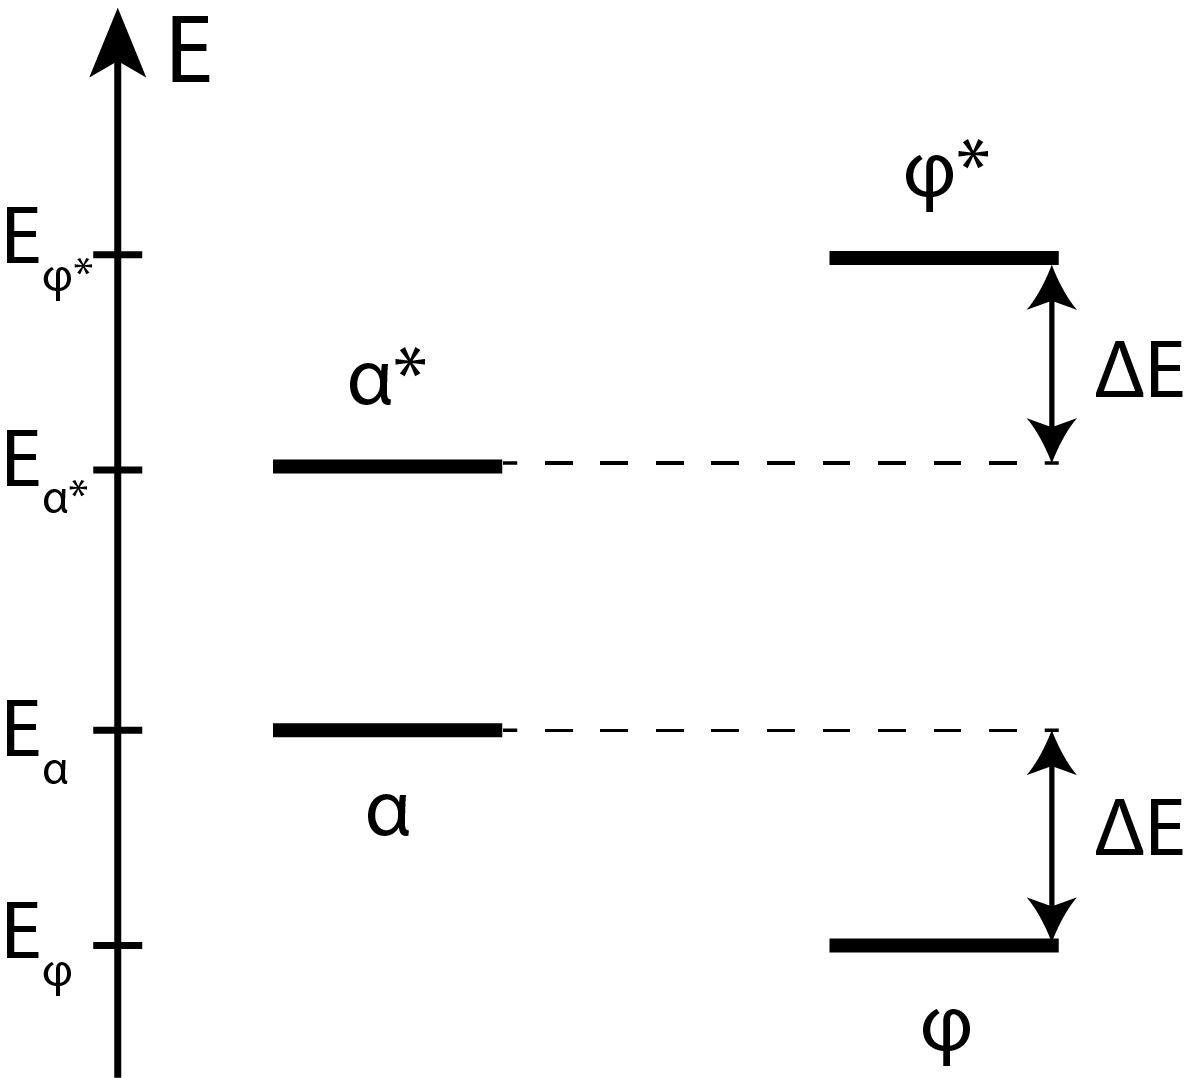
\includegraphics[width=0.3\linewidth]{Fig1.png}
\caption{Энергетическая диаграмма для орбиталей из двух базисных наборов: $(\alpha, \alpha^{\star})$ и $(\phi, \phi^{\star})$.}
\label{fig:fig1}
\end{figure}

Будем считать, что нам дана матрица Фока в базисе орбиталей $\alpha$ и $\alpha^\star$:

\begin{equation}
    \textbf{F} = 
    \begin{pmatrix}
        E_{\alpha} & F_{12} \\
        F_{12} & E_{\alpha^{\star}}
    \end{pmatrix},
\end{equation}
где $E_{\alpha}$ и $E_{\alpha^{\star}}$ - энергии орбиталей.

А в базисе молекулярных орбиталей $\phi$ и $\phi^{\star}$ матрица Фока должна быть диагональной:

\begin{equation}
    \textbf{F} = 
    \begin{pmatrix}
        E_{\phi} & 0 \\
        0 & E_{\phi^{\star}}
    \end{pmatrix},
\end{equation}
где $E_{\phi}$ и $E_{\phi^{\star}}$ - энергии МО.

Задача, которую решают теорией возмущений, заключается в нахождении энергии взаимодействия орбиталей $\alpha$ и $\alpha^\star$, то есть разности энергий занятых орбиталей до и после взаимодействия:

\begin{equation}
    \Delta E = \vert E_{\phi} - E_{\alpha} \vert
\end{equation}

Для применения теории возмущений будем считать, что в нулевом приближении орбитали $\alpha$ и $\alpha^\star$ не взаимодействуют, то есть невозмущенная матрица Фока в базисе $\alpha$ и $\alpha^\star$ имеет вид:

\begin{equation}
    \textbf{F}_{0} = 
    \begin{pmatrix}
        E_{\alpha} & 0 \\
        0 & E_{\alpha^{\star}}
    \end{pmatrix},
\end{equation}

Тогда вид матрицы оператора возмущения $\textbf{V}$ можно получить вычитанием невозмущенной матрицы $\textbf{F}_0$ из невозмущенной $\textbf{F}$:

\begin{equation}
    \textbf{V} = 
    \textbf{F} - \textbf{F}_0 =
    \begin{pmatrix}
        E_{\alpha} & F_{12} \\
        F_{12} & E_{\alpha^{\star}}
    \end{pmatrix}
    -
    \begin{pmatrix}
        E_{\alpha} & 0 \\
        0 & E_{\alpha^{\star}}
    \end{pmatrix}
    =
    \begin{pmatrix}
        0 & F_{12} \\
        F_{12} & 0
    \end{pmatrix}
\end{equation}

\subsection{Поправка первого порядка}

Пользуясь формулами с п.1 получаем, что 

\begin{equation}
    E_{\alpha}^{(1)} = \braket{\alpha|\textbf{V}|\alpha}.
\end{equation}

И далее записываем $\alpha$ и $\textbf{V}$ в базисе орбиталей $\alpha$ и $\alpha^\star$:

\begin{equation}
    \braket{\alpha|\textbf{V}|\alpha} = 
    \begin{pmatrix}
        1 & 0
    \end{pmatrix}
    \begin{pmatrix}
        0 & F_{12} \\
        F_{12} & 0
    \end{pmatrix}
    \begin{pmatrix}
        1 \\
        0
    \end{pmatrix}
    = 0.
\end{equation}

Получается, что поправка первого порядка равна нулю, потому что диагональные элементы матрицы возмущения нулевые.

\subsection{Поправка второго порядка}

Пользуясь формулами с п.1 получаем, что 

\begin{equation}
    E_{\alpha}^{(2)} = \frac{|\braket{\alpha^{\star}|\textbf{V}|\alpha}|^2}{E_{\alpha} - E_{\alpha^{\star}}}.
\end{equation}

Распишем чему равен $\braket{\alpha^{\star}|\textbf{V}|\alpha}$ в базисе $\alpha$ и $\alpha^\star$:

\begin{equation}
    \braket{\alpha^{\star}|\textbf{V}|\alpha} = 
    \begin{pmatrix}
        0 & 1
    \end{pmatrix}
    \begin{pmatrix}
        0 & F_{12} \\
        F_{12} & 0
    \end{pmatrix}
    \begin{pmatrix}
        1 \\
        0
    \end{pmatrix}
    = F_{12}.
\end{equation}

В итоге получаем приближенную формулу для энергии, на которую понижается $E_\alpha$ при взаимодействии с $\alpha^\star$:

\begin{equation}
    \Delta E = E_{\phi} - E_{\alpha} \approx \frac{|\braket{\alpha^{\star}|\textbf{V}|\alpha}|^2}{E_{\alpha} - E_{\alpha^{\star}} }
    = -\frac{F_{12}^2}{E_{\alpha^{\star}} - E_{\alpha}}.
    \label{eq:secondorder}
\end{equation}

Умножением этой энергии на занятость орбитали приходим к привычной формуле энергии взаимодействия NBO:

\begin{equation}
    E(2) = - n_{\alpha} \frac{F_{ij}^2}{E_{\alpha^{\star}}-E_{\alpha}}.
\end{equation}

\section{Другой способ расчета энергии взаимодействия орбиталей}

Здесь будет рассмотрен более простой способ нахождения энергии взаимодействия орбиталей на примере системы из п.2. Считаем, что нам дана матрица Фока в базисе орбиталей $\alpha$ и $\alpha^\star$:

\begin{equation}
    \textbf{F} = 
    \begin{pmatrix}
        E_{\alpha} & F_{12} \\
        F_{12} & E_{\alpha^{\star}}
    \end{pmatrix},
\end{equation}
где $E_{\alpha}$ и $E_{\alpha^{\star}}$ - энергии орбиталей.

Чтобы найти энергию взаимодействия между $\alpha$ и $\alpha^\star$ нужно вывести формулу для собственных значений оператора $\textbf{F}$. Проделав символьный расчет,  получаем, что найдется некоторый базис, в котором матрица нашего оператора Фока будет иметь приведенный ниже диагональный вид:

\begin{gather}
    \textbf{F} = 
    \begin{pmatrix}
        E_{\alpha} & F_{12} \\
        F_{12} & E_{\alpha^{\star}}
    \end{pmatrix}
    \xrightarrow{\text{For some}\ \textbf{T}}
    \textbf{F}' = \textbf{T}^{-1} \textbf{F} \textbf{T} = 
    \begin{pmatrix}
        E_{\phi} & 0 \\
        0 & E_{\phi^{\star}}
    \end{pmatrix},\notag\\
    E_{\phi} = \frac{1}{2} \cdot \left( E_{\alpha} + E_{\alpha^{\star}} - \sqrt{4F_{12}^2 + \left( E_{\alpha^{\star}} - E_{\alpha}\right)^2 } \right) \notag\\
    E_{\phi^{\star}} = \frac{1}{2} \cdot \left( E_{\alpha} + E_{\alpha^{\star}} + \sqrt{4F_{12}^2 + \left( E_{\alpha^{\star}} - E_{\alpha}\right)^2 } \right)
    \label{eq:myneweq}
\end{gather}
где $E_{\phi}$ и $E_{\phi^{\star}}$ - энергии МО, получившихся при взаимодействии между $\alpha$ и $\alpha^\star$.

Посмотрим на некоторые свойства полученных формул.

\subsection{Связь с теорией возмущений}

Оказалось, что из \eqref{eq:myneweq} можно вывести формулу второго порядка теории возмущений \eqref{eq:secondorder}. Для этого можно использовать следующую эквивалентность:

\begin{equation}
    \sqrt{1+x} = 1 + \frac{1}{2} x + O(x^2).
\end{equation}

Ниже приведен полный вывод для занятой орбитали. Дополнительно принимаем, что $E_{\alpha} \leq E_{\alpha^{\star}}$.

\begin{gather} \label{eq:case1start}
    E_{\phi} = \frac{1}{2} \cdot \left( E_{\alpha} + E_{\alpha^{\star}} - \sqrt{4F_{12}^2 + \left( E_{\alpha^{\star}} - E_{\alpha}\right)^2 } \right) =  \\ 
    = \frac{1}{2} \cdot \left( E_{\alpha} + E_{\alpha^{\star}} - \left( E_{\alpha^{\star}} - E_{\alpha}\right) \sqrt{ 1 + \frac{4 F_{12}^2}{\left( E_{\alpha^{\star}} - E_{\alpha}\right)^2} } \right) = \\
    = \frac{1}{2} \cdot \left( E_{\alpha} + E_{\alpha^{\star}} - \left( E_{\alpha^{\star}} - E_{\alpha}\right) \left(1 + \frac{2 F_{12}^2}{\left( E_{\alpha^{\star}} - E_{\alpha}\right)^2} + O\left(\frac{F_{12}^4}{\left( E_{\alpha^{\star}} - E_{\alpha}\right)^4}\right) \right) \right) = \\
    = E_{\alpha} - \frac{F_{12}^2}{E_{\alpha^{\star}} - E_{\alpha}} + O\left(\frac{F_{12}^4}{\left( E_{\alpha^{\star}} - E_{\alpha}\right)^3}\right) \label{eq:case1end}
\end{gather} 

Получается, что при достаточно малых $F_{ij}$ и достаточно больших $\Delta E$ расчеты по второму порядку теории возмущений дают такие же результаты, как и по формулам \eqref{eq:myneweq}. И наоборот, при увеличении $F_{ij}$ или уменьшении $\Delta E$ различие между энергиями взаимодействий получаемыми по формулам \eqref{eq:secondorder} и \eqref{eq:myneweq} растет, как $O(F_{ij}^4)$ и $O(\Delta E ^ {-3})$.

\subsection{Другое приближение}

По сути, преобразования \eqref{eq:case1start}--\eqref{eq:case1end} были сделаны в приближении $F_{12} \ll E_{\alpha^{\star}} - E_{\alpha}$. Оказывается, что симметричность исходных формул \eqref{eq:myneweq} позволяет по аналогии вывести энергии взаимодействия орбиталей в приближении $F_{12} \gg E_{\alpha^{\star}} - E_{\alpha}$.

\begin{gather} \label{eq:case2start}
    E_{\phi} = \frac{1}{2} \cdot \left( E_{\alpha} + E_{\alpha^{\star}} - \sqrt{4F_{12}^2 + \left( E_{\alpha^{\star}} - E_{\alpha}\right)^2 } \right) =  \\ 
    = \frac{1}{2} \cdot \left( E_{\alpha} + E_{\alpha^{\star}} - 2 F_{12} \sqrt{ 1 + \frac{\left( E_{\alpha^{\star}} - E_{\alpha}\right)^2}{4 F_{12}^2} } \right) = \\
    = \frac{1}{2} \cdot \left( E_{\alpha} + E_{\alpha^{\star}} - 2 F_{12} \left( 1 + \frac{\left( E_{\alpha^{\star}} - E_{\alpha}\right)^2}{8 F_{12}^2} + O\left(  \frac{\left( E_{\alpha^{\star}} - E_{\alpha}\right)^4}{F_{12}^4} \right)  \right) \right) = \\
    = \frac{E_{\alpha} + E_{\alpha^{\star}}}{2} - \left( F_{12} + \frac{\left( E_{\alpha^{\star}} - E_{\alpha}\right)^2}{8 F_{12}} \right) + O\left( \frac{\left( E_{\alpha^{\star}} - E_{\alpha}\right)^4}{F_{12}^3} \right)
    \label{eq:case2end}
\end{gather} 

Резюмируя два рассмотренных случая:

1) $F_{12} \ll E_{\alpha^{\star}} - E_{\alpha}$. В первом приближении орбитали не взаимодействуют (точно верно при $F_{12} = 0$):

\begin{gather} 
    E_{\phi} = E_{\alpha} \notag\\
    E_{\phi^{\star}} = E_{\alpha^{\star}}
\end{gather}

Во втором приближении (см. \eqref{eq:case1start}--\eqref{eq:case1end}) энергия взаимодействия соответствует теории возмущений второго порядка:

\begin{gather} 
    E_{\phi} = E_{\alpha} - \frac{F_{12}^2}{E_{\alpha^{\star}}-E_{\alpha}}\notag\\
    E_{\phi^{\star}} = E_{\alpha^{\star}} + \frac{F_{12}^2}{E_{\alpha^{\star}}-E_{\alpha}}
\end{gather}

2) $F_{12} \gg E_{\alpha^{\star}} - E_{\alpha}$. Первое приближение соответствует взаимодействию двух вырожденных по энергии орбиталей, в таком случае энергия взаимодействия составляет $F_{12}$:

\begin{gather} 
    E_{\alpha} = E_{\alpha^{\star}} \notag\\
    E_{\phi,\phi^{\star}} = E_{\alpha} \pm F_{12}
\end{gather}

Второе приближение (см. \eqref{eq:case2start}--\eqref{eq:case2end}) дает зависимость энергии взаимодействия от разности $E_{\alpha^{\star}} - E_{\alpha}$, при её малых значениях. Из \eqref{eq:case2end} можно вывести:

\begin{gather} 
    E_{\phi} = E_{\alpha} - \left( F_{12} - \frac{E_{\alpha^{\star}} - E_{\alpha}}{2} \left( 1 - \frac{E_{\alpha^{\star}} - E_{\alpha}}{4 F_{12}} \right) \right) \notag\\
    E_{\phi^{\star}} = E_{\alpha^{\star}} + \left( F_{12} - \frac{E_{\alpha^{\star}} - E_{\alpha}}{2} \left( 1 - \frac{E_{\alpha^{\star}} - E_{\alpha}}{4 F_{12}} \right) \right)
    \label{eq:secorder2}
\end{gather}

Химическая логика, что энергия взаимодействия должна уменьшаться при увеличении $E_{\alpha^{\star}} - E_{\alpha}$ подтверждается выражением \eqref{eq:secorder2}, если учесть, что $F_{12} \gg E_{\alpha^{\star}} - E_{\alpha} \Rightarrow \frac{E_{\alpha^{\star}} - E_{\alpha}}{4 F_{12}} \ll 1$ и принять $E_{\alpha^{\star}} - E_{\alpha} > 0$. 

\subsection{Физический смысл $F_{ij}$}

\begin{figure}[h]
    \centering
    \captionsetup{justification=centering}
    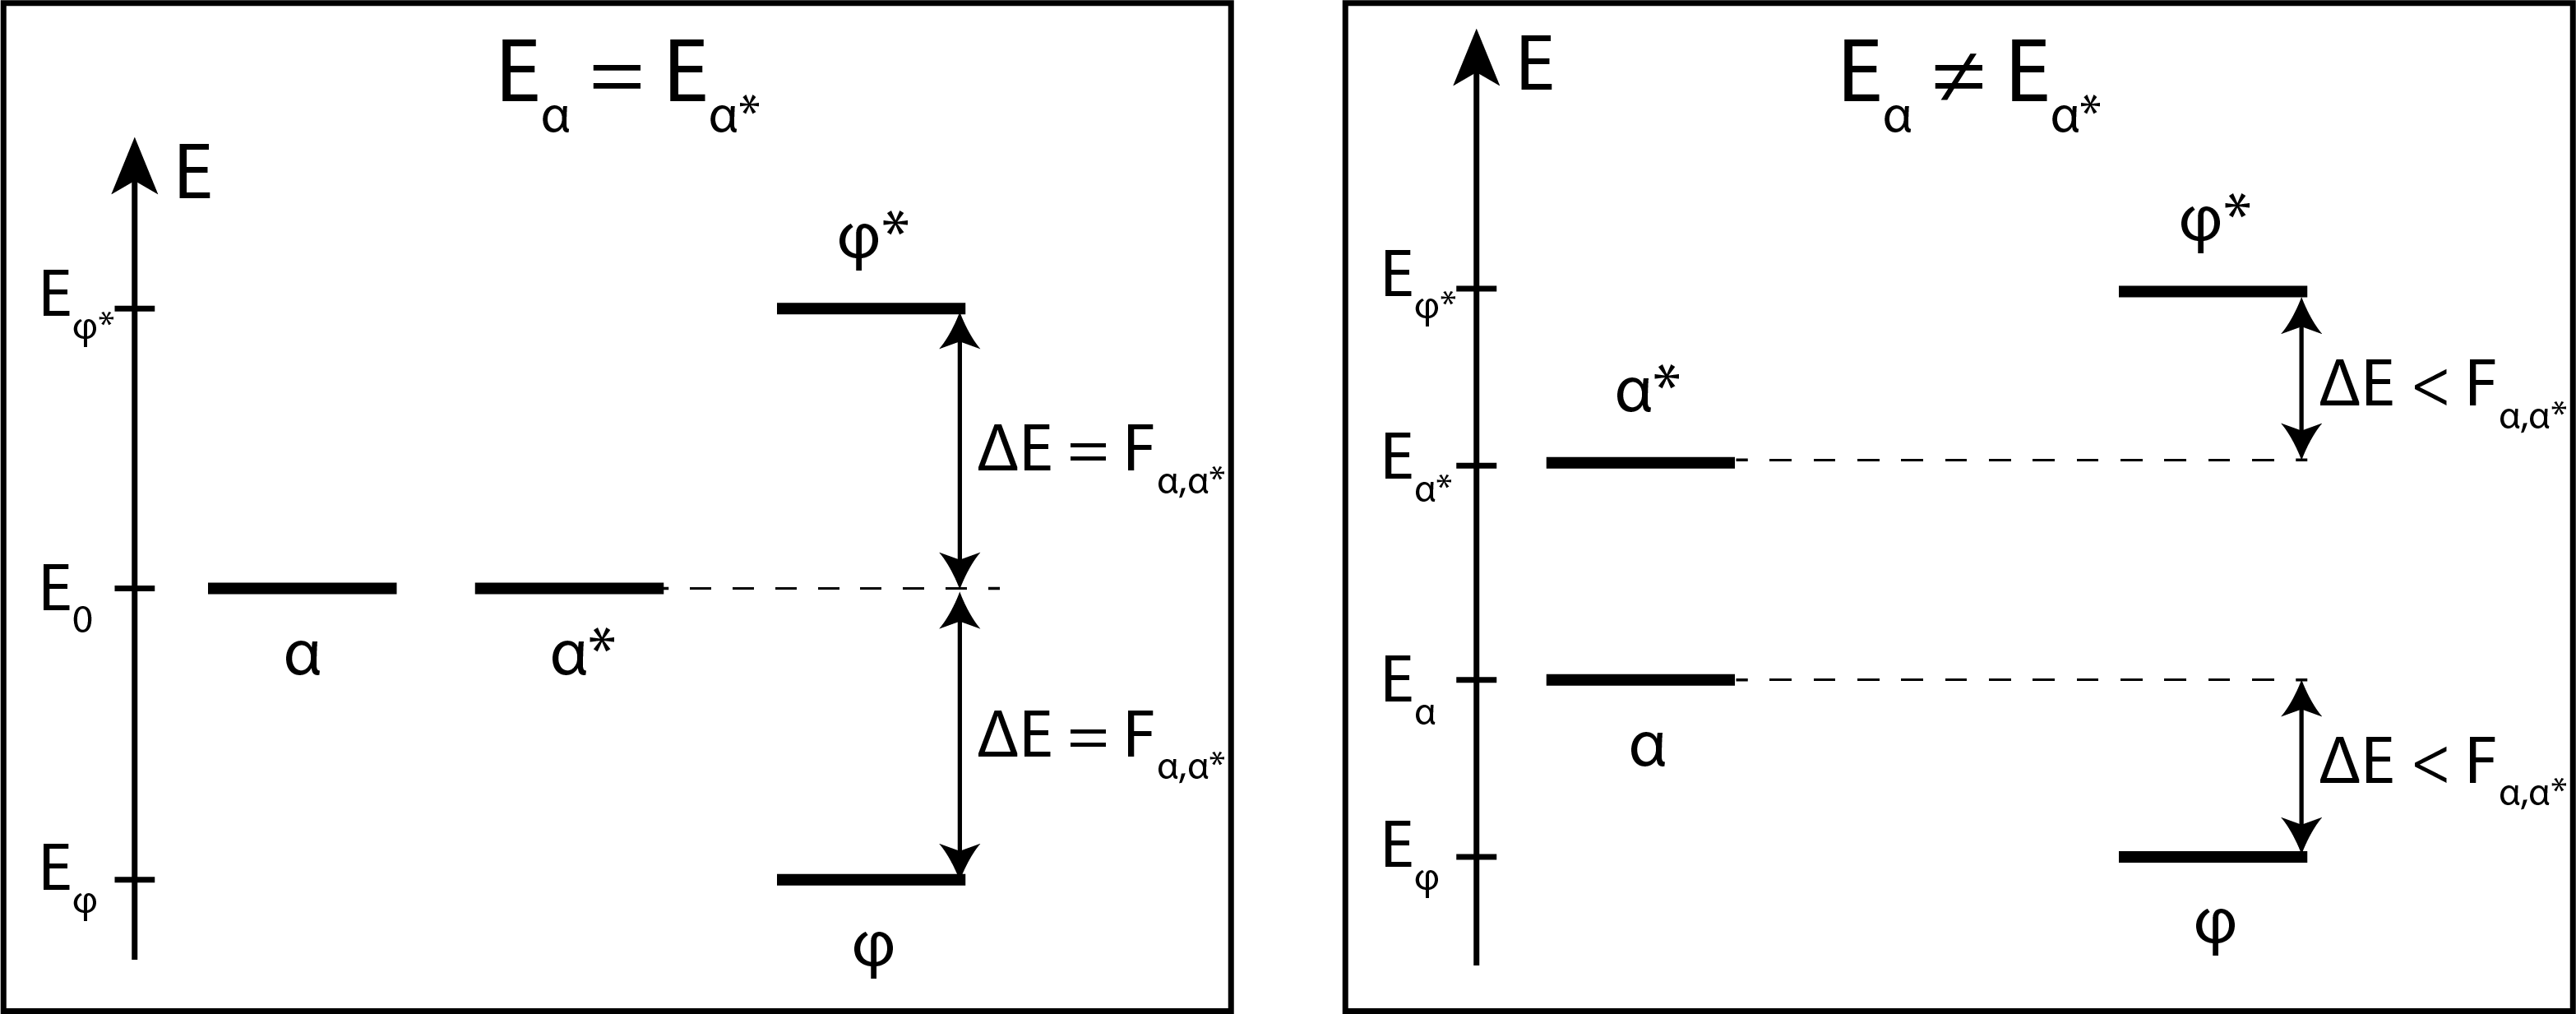
\includegraphics[width=1\linewidth]{Fig2.png}
    \caption{Иллюстрация физического смысла недиагональных элементов матрицы Фока.}
    \label{fig:fig2}
    \end{figure}

В итоге из \eqref{eq:secorder2} стало понятно, что физический смысл $F_{ij}$ проявляется при анализе случая $F_{12} \gg E_{\alpha^{\star}} - E_{\alpha}$ и его можно сформулировать в двух вариантах:
 
\fbox{\begin{minipage}{45em}
    \textbf{1. Недиагональный элемент матрицы Фока - это энергия, с которой взаимодействовали бы орбитали, если бы у них были одинаковые энергии (см. левую часть рисунка \ref{fig:fig2}).}
\end{minipage}}

\fbox{\begin{minipage}{45em}
    \textbf{2. Недиагональный элемент матрицы Фока - это максимально возможная энергия взаимодействия орбиталей, независимо от их собственных энергий (см. правую часть рисунка \ref{fig:fig2}).}
\end{minipage}}

\end{document}
